\documentclass[draft,linenumbers]{agujournal}
\draftfalse
\usepackage{hyperref}
\usepackage[export]{adjustbox}
\addtolength{\oddsidemargin}{-.875in}
\addtolength{\evensidemargin}{-.875in}
	
\hypersetup{
    colorlinks=true,
    linkcolor=blue,
    filecolor=magenta,      
    urlcolor=cyan,
}

\journalname{Journal of Advances in Modeling Earth Systems (JAMES)}

\begin{document}


 \begin{figure}[h]
    % \centering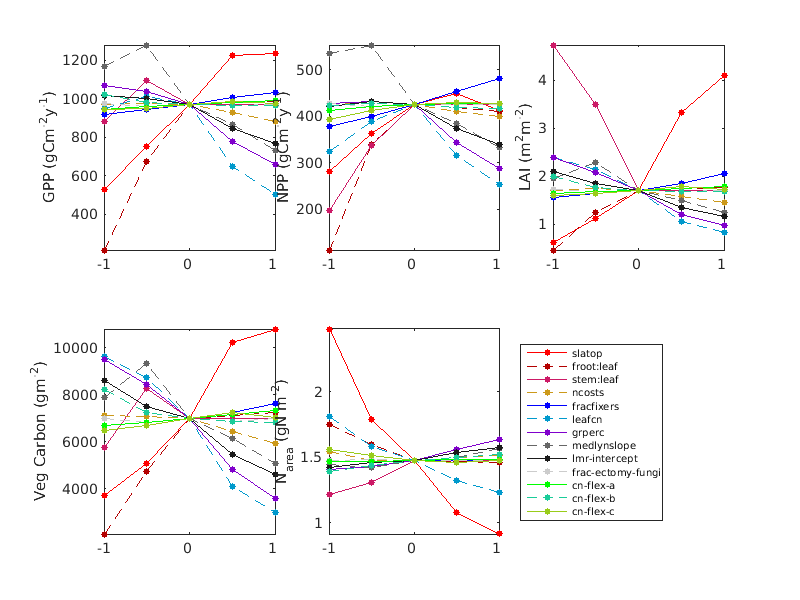
\includegraphics[width=0.5\textwidth, right]{lion-lo9
     \includegraphics[width=1.3\textwidth, left]{matlab/figures/NOVc_STATE_1CLM50defpft_trans_1x1pt_US-NR1_ens_MIC_y1_2012.png}
     \caption{Response of control model states and fluxes to parameter perturbation across -1 to +1 range of parameter variation at Niwot Ridge.}
     \label{NR1 state}
 \end{figure}
 

  \begin{figure}[h]
    % \centering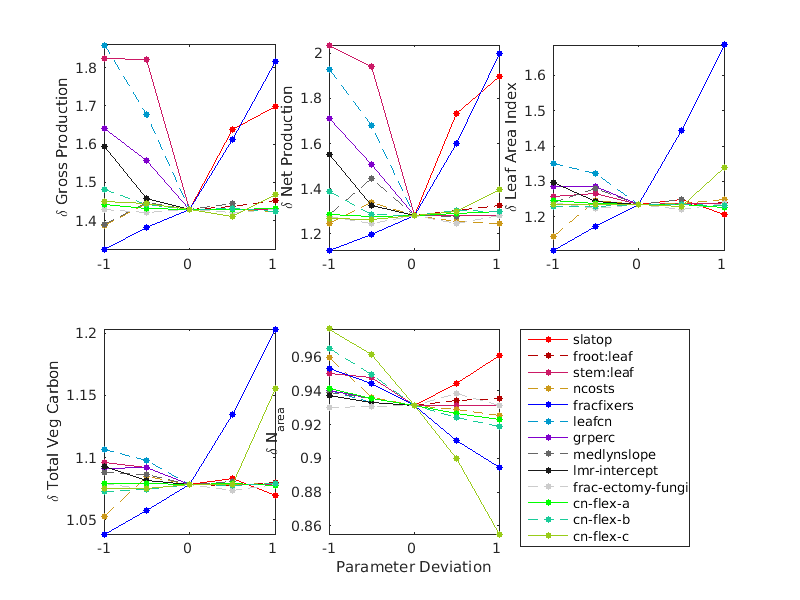
\includegraphics[width=0.5\textwidth, right]{lion-lo9
     \includegraphics[width=1.3\textwidth, left]{matlab/figures/NOVc_FERT_1CLM50defpft_celev_1x1pt_US-NR1_ens_MIC_p1_2012.png}
     \caption{Influence of parametric variation (over the range tested: -1 to +1) on the influence of 15 years of CO$_{2}$ fertilization (550ppm) at Niwot Ridge}
     \label{NR1 celev}
  \end{figure}
  
  \begin{figure}[h]
    % \centering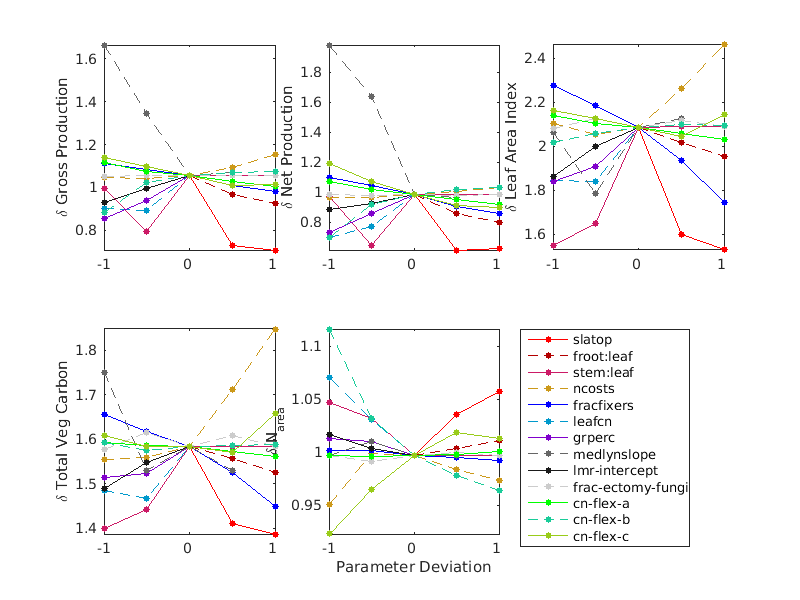
\includegraphics[width=0.5\textwidth, right]{lion-lo9
     \includegraphics[width=1.3\textwidth, left]{matlab/figures/NOVc_FERT_1CLM50defpft_ndep_1x1pt_US-NR1_ens_MIC_p1_2012.png}
     \caption{Influence of parametric variation (over the range tested: -1 to +1) on the influence of 15 years of Nitrogen fertilization (+5 kgN m$^{2}$ y$^{-1}$) at Niwot Ridge}
     \label{NR1 ndep}
  \end{figure}
  
      
 \begin{figure}[h]
     \centering
     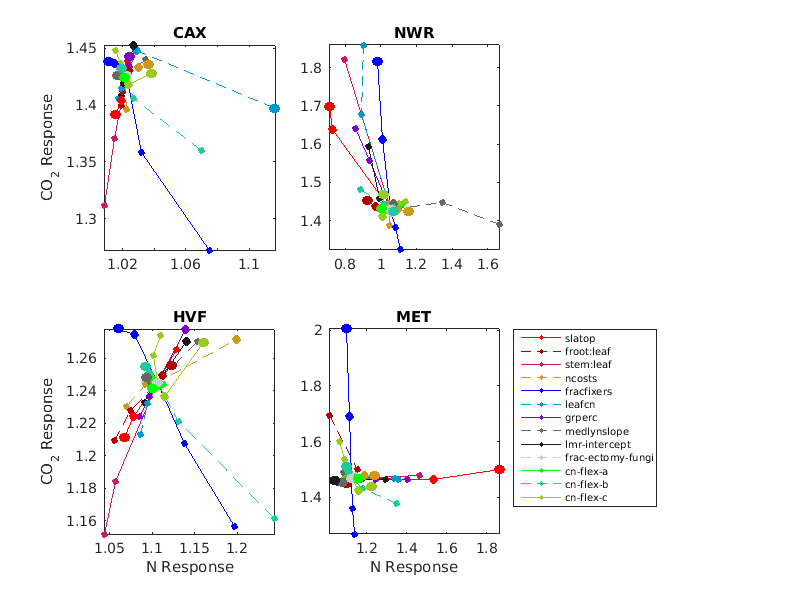
\includegraphics[width=1.55\textwidth, left]{matlab/figures/NOVc_CNdep_GPP1__p2012.png}
     \caption{Influence of parameteric variation on the impact of 15 years of CO$_{2}$ and N fertilization on gross primary productivity (GPP), across the Caxiuan\~a (CAX), Niwot Ridge (NWR), Harvard Forest (HVF) and Metolious MET) sites. }
     \label{GPP CO2 and N respones 2001}
  \end{figure}
  
 \begin{figure}[h]
     \centering
     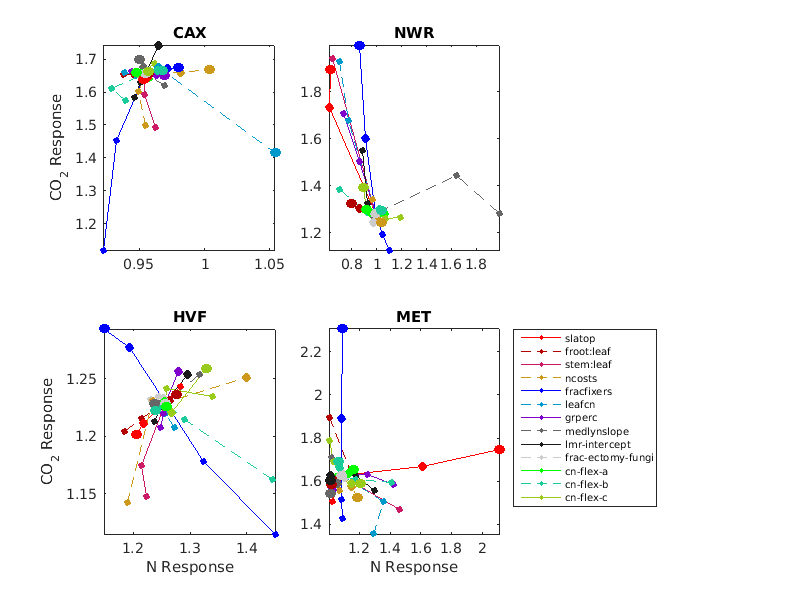
\includegraphics[width=1.55\textwidth, left]{matlab/figures/NOVc_CNdep_NPP1__p2012.png}
     \caption{Influence of parametric variation on the impact of 15 years of CO$_{2}$ and N fertilization on net primary productivity (NPP), across the Caxiuan\~a (CAX), Niwot Ridge (NWR), Harvard Forest (HVF) and Metolious MET) sites.}
     \label{NPP CO2 and N respones 2001}
  \end{figure}
  
  \begin{figure}[h]
     \centering
     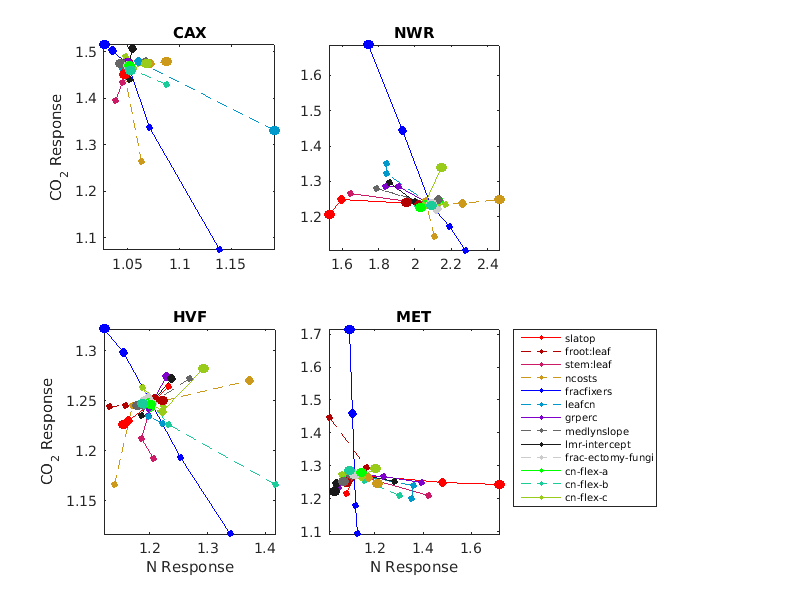
\includegraphics[width=1.55\textwidth, left]{matlab/figures/NOVc_CNdep_TLAI1__p2012.png}
     \caption{Influence of parametric variation on the impact of 15 years of CO$_{2}$ and N fertilization on leaf area index (LAI), across the Caxiuan\~a (CAX), Niwot Ridge (NWR), Harvard Forest (HVF) and Metolious MET) sites.}
     \label{LAI CO2 and N respones 2001}
  \end{figure}
  
 
    
 
\end{document}